\documentclass{bioinfo}
\copyrightyear{2015} \pubyear{2015}

\usepackage{url}

\access{Advance Access Publication Date: Day Month Year}
\appnotes{Genome analysis}

\begin{document}
\firstpage{1}

\title[Parallelizing workflows with Cannoli]{Automatically parallelizing bioinformatics workflows with Cannoli}
\author[Heuer \textit{et~al}.]{Michael~Heuer\,$^{\text{\sfb 1,}*}$ and Frank~Austin~Nothaft\,$^{\text{\sfb 2}}$}
\address{$^{\text{\sf 1}}$Department of Electrical Engineering and Computer Sciences, University of California, Berkeley, CA 94720, USA and \\
$^{\text{\sf 2}}$Databricks, Inc., San Francisco, CA 94105, USA}

\corresp{$^\ast$To whom correspondence should be addressed.}

\history{Received on XXXXX; revised on XXXXX; accepted on XXXXX}

\editor{Associate Editor: XXXXXXX}

\abstract{\textbf{Motivation:} Due to their computational complexity, secondary bioinformatics
  pipelines can take more than a day to run. While accelerated implementations of popular tools
  like the GATK exist, these implementations are typically proprietary and cover a limited set
  of bioinformatics workflows. Bioinformaticians frequently resort to manual methods to run an
  analysis in parallel, such as writing scripts that split by genomic locus. These scripts add
  complexity to maintaining a pipeline and may not achieve optimal scaling.\\
\textbf{Results:} Cannoli provides a user-friendly API and CLI that automatically parallelizes
  21 common bioinformatics. Cannoli builds on top of Apache Spark and ADAM's pipe API, which
  provides fault-tolerant execution portably across a local machine, an on-premises compute farm,
  and cloud computing. Benchmarking on common variant calling and single-cell RNA-seq quantification
  pipelines demonstrates that Cannoli can reduce workflow runtime by FIXME$\times$\\
\textbf{Availability:} Cannoli is open-source software, distributed under an Apache 2 license.
Cannoli is available from \url{https://github.com/bigdatagenomics/cannoli}.\\
\textbf{Contact:} \href{heuermh@berkeley.edu}{heuermh@berkeley.edu}\\
\textbf{Supplementary information:} Supplementary data are available at \textit{Bioinformatics}
online.}

\maketitle

\section{Introduction}

\begin{itemize}
\item Bioinformatics workflows are slow and complex.
  \begin{itemize}
  \item Often involve many tools chained together, running on a single node
  \item Bioinformaticians often rely on one-off scripts to parallelize tools
  \item These scripts add complexity to a workflow and make workflows liable to fail
  \item Since we are often parallelizing by genomic locus, we can automatically parallelize most tools
  \end{itemize}
\item Cannoli provides automatic parallelization of bioinformatics workflows in an easy-to-use and
  composable framework
  \begin{itemize}
  \item Cannoli is built on top of Apache Spark~\citep{zaharia12} and ADAM~\citep{massie13, nothaft15}
  \item Cannoli supports 21 common bioinformatics tools using ADAM's pipe API~\citep{nothaft17}, which
    allows a user to run tools in parallel across a cluster, with built-in fault tolerance
  \item Each tool invocation takes a single line of code, and Cannoli uses Docker to simplify tool
    installation~\citep{daveiga17}
  \end{itemize}
\item In this application note, we walk through Cannoli's architecture and evaluate it on two pipelines
  \begin{itemize}
  \item We implement a germline variant calling use case using BWA and FreeBayes through Cannoli
  \item We implement an end-to-end scRNA-seq pipeline using Cannoli and Apache Spark SQL
  \end{itemize}
\end{itemize}

%\enlargethispage{12pt}

\section{Approach}

\begin{itemize}
\item Cannoli provides both an API and a CLI for running a set of 21 bioinformatics tools
  \begin{itemize}
  \item Cannoli wraps each tool in a \texttt{CannoliFn}, a one-line command that
    can be called in Scala to run the command
  \item A \texttt{CannoliFn} transforms an ADAM~\citep{massie13, nothaft15} dataset
    into a new ADAM dataset
  \item Inside a \texttt{CannoliFn}, we build a command for the tool we are running,
    and pass this command to ADAM's pipe API
  \end{itemize}
\end{itemize}

\begin{figure}[!tpb]
\centerline{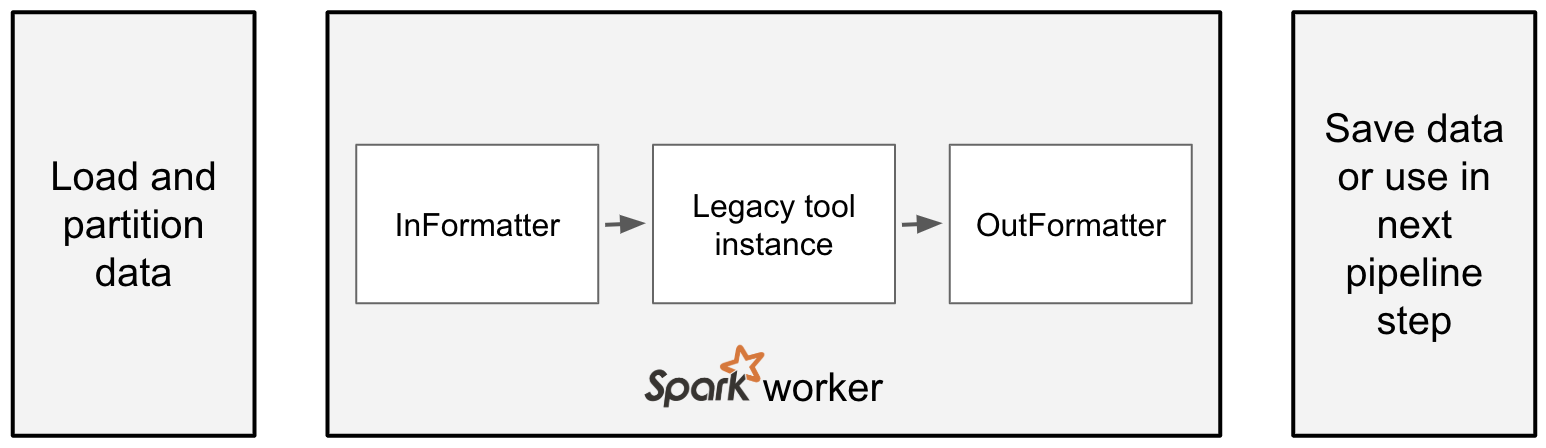
\includegraphics[width=0.95\linewidth]{pipe.png}}
\caption{Schematic of ADAM's pipe function.}\label{fig:pipe}
\end{figure}

\begin{itemize}
\item This architecture makes it very easy to support a large number of tools
  \begin{itemize}
  \item \texttt{CannoliFn}s have access to a \texttt{CommandBuilder}, which strings
    together arguments for a bioinformatics tool according to configured parameters
  \item \texttt{CommandBuilder}s also abstract away whether the command is run using
    a Docker container---defaulting to a BioContainer~\citep{daveiga17}---or a
    pre-installed executable
  \item Once a \texttt{CannoliFn} is built, it is accessible on top of an ADAM dataset
    and a thin wrapper exposes the function as a command-line tool
  \end{itemize}
\item The simplicity of this approach has allowed us to add support for the 21 tools
  described in Table~\ref{tab:tools}.
\end{itemize}

\begin{table}[!t]
\processtable{Tools supported in Cannoli\label{tab:tools}}{\begin{tabular}{|l|l|}\toprule Aligners & \\\midrule
 & bowtie \\
 & bowtie2 \\
 & bwa \\
 & gem \\
 & minimap2 \\
 & star \\\midrule
Variant Callers & \\
 & freebayes \\
 & samtools mpileup \\\midrule
Variant Manipulators & \\
 & snpeff \\
 & vep \\
 & bcftools \\
 & vt \\\midrule
Other & \\
 & bedtools \\
 & blastn \\
 & magic-blast \\
    \\\botrule
\end{tabular}}{}
\end{table}

\begin{methods}
\section{Methods}

Text Text Text Text Text Text  Text Text Text Text Text Text Text
Text Text  Text Text Text Text Text Text.
Figure~2\vphantom{\ref{fig:02}} shows that the above method  Text
Text Text Text  Text Text Text Text Text Text  Text Text.
\citealp{Boffelli03} might want to know about  text text text text
Text Text Text Text Text Text Text Text Text Text Text Text Text
Text Text  Text Text Text Text Text Text.
Figure~2\vphantom{\ref{fig:02}} shows that the above method  Text
Text Text Text Text Text Text Text Text Text  Text Text.
\citealp{Boffelli03} might want to know about text text text text
Text Text Text Text Text Text  Text Text Text Text Text Text Text
Text Text Text Text Text Text Text Text.
Figure~2\vphantom{\ref{fig:02}} shows that the above method  Text
Text Text Text Text Text Text Text Text Text  Text Text.
\citealp{Boffelli03} might want to know about text text text
text\vspace*{1pt}

\end{methods}

\section{Discussion}

\begin{itemize}
\item We see Cannoli as an alternative to a workflow manager, but not inherently
  competitive
  \begin{itemize}
  \item Large number of existing workflow runners, many of which focus on metadata
    capture, some of which extend existing programming paradigms, some of which
    introduce new domain-specific languages, none of which focus on automatic
    parallelization
  \item Cannoli does not focus on metadata capture and extends an existing
    programming paradigm (ADAM/Scala), but instead provides automated parallelization
  \item Cannoli's API enables users to rapidly build and run pipelines that include
    ad hoc manipulations of data (e.g., align reads and then filter out low map-Q
    reads, call variants and apply region-specific predicates)
  \item This is useful for rapid experimentation, and eliminates common workflow
    smells (e.g., pipe VCF through \texttt{grep} to do variant filtration)
  \item Cannoli's CLI enables straightforward integration with existing workflow
    managers
  \end{itemize}
\end{itemize}

\section{Conclusion}

\begin{itemize}
\item Cannoli improves the latency of bioinformatics tools, while improving
  ease of use and reproducibility
  \begin{itemize}
  \item Cannoli's API allows users to run 21 tools, with a single line of
    code per tool, which allows users to simply compose workflows
  \item These APIs are also exposed through a command-line, enabling easy
    interoperability with traditional bioinformatics workflows
  \item These APIs can easily be extended to support new bioinformatics tools
  \item We have demonstrated how the API and CLI can be used to accelerate
    variant calling and scRNA quantification workflows by FIXME$\times$
  \end{itemize}
\end{itemize}

\section*{Acknowledgements}

Work on Cannoli started at the Bioinformatics Open Source Conference
codefest, and was encouraged along by members of the Big Data Genomics
project, as well as the broader open-source bioinformatics community.

\section*{Funding}

This work was supported by NSF CISE Expeditions Award CCF-1139158, LBNL Award 7076018, and DARPA XData Award FA8750-12-2-0331, NIH BD2K Award 1-U54HG007990-01, NIH Cancer Cloud Pilot Award HHSN261201400006C and gifts from Amazon Web Services, Google, SAP,  The Thomas and Stacey Siebel Foundation, Adatao, Adobe, Apple, Inc., Blue Goji, Bosch, C3Energy, Cisco, Cray, Cloudera, EMC, Ericsson, Facebook, Guavus, Huawei, Intel, Microsoft, NetApp, Pivotal, Samsung, Splunk, Virdata, VMware, and Yahoo!.

%\bibliographystyle{natbib}
%\bibliographystyle{achemnat}
%\bibliographystyle{plainnat}
%\bibliographystyle{abbrv}
%\bibliographystyle{bioinformatics}
%
%\bibliographystyle{plain}
%
%\bibliography{Document}


\bibliographystyle{natbib}
\bibliography{main}
\end{document}
